
%(BEGIN_QUESTION)
% Copyright 2010, Tony R. Kuphaldt, released under the Creative Commons Attribution License (v 1.0)
% This means you may do almost anything with this work of mine, so long as you give me proper credit

Under en «As-Found»-analyse av en reguleringsventil med smart posisjonerer registrerer en instrumenttekniker denne uvanlige ventilsignaturen:

$$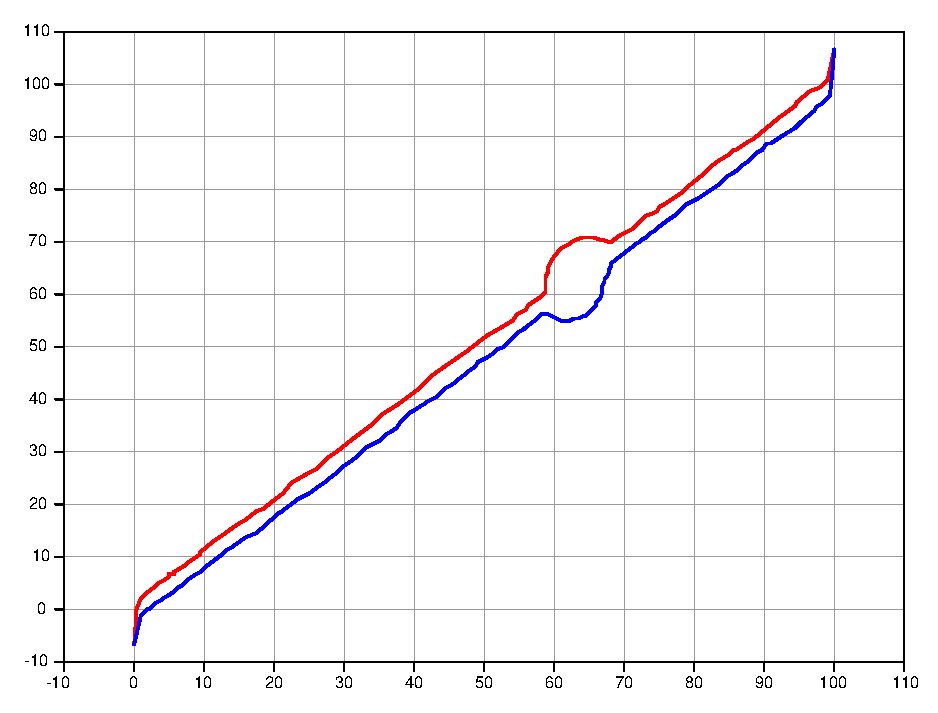
\includegraphics[width=15.5cm]{i00746x01.eps}$$

Hva tror du de uvanlige «kulene» i kurvene representerer? Hvilket/hvilke fysiske problem(er) bør teknikeren begynne å lete etter når ventilen undersøkes?

\vskip 20pt \vbox{\hrule \hbox{\strut \vrule{} {\bf Forslag til sokratisk diskusjon} \vrule} \hrule}

\begin{itemize}
\item{} En nyttig problemløsningsteknikk ved alle scenarier med grafer er å la grafen «fortelle deg» hva som skjer trinn for trinn over tid når du følger den fra ett ytterpunkt til det andre. Prøv dette: start i nedre venstre hjørne, følg den øvre (røde) kurven steg for steg som om du spiller av ventilåpningen over tid, og tolk grafen i lys av spindelposisjon og aktuatortrykk (påført kraft). Beskriv hva grafen «forteller» deg når du følger den fra den ene enden til den andre.
\end{itemize}

\underbar{file i00746}
%(END_QUESTION)



%(BEGIN_ANSWER)

«Kulen» indikerer en brå endring i friksjonskraft fra omtrent 58\% til 68\% av ventilspindelens vandring, men normal friksjon gjennom resten av vandringen.

%(END_ANSWER)





%(BEGIN_NOTES)

Teknikeren bør begynne å lete etter noe unormalt på ventilspindelen eller ventilsatsen (hvis den er bur-guidet) som skaper friksjon i dette vandringsområdet. Det kan for eksempel være korrosjon på ett punkt av spindelen (som gnir mer mot pakkboksen mellom 58\% og 68\% vandring), eller at stempelet gnisser mot buret i ett område.

%INDEX% Sluttkontrollelementer, ventil: diagnostisk signatur for pneumatisk aktuator

%(END_NOTES)


